\textbf{COLUNI 2019 -- Questão 24}\par\medskip Um bloco de madeira cúbico está em repouso sobre uma tábua inclinada, como é apresentado na figura a seguir:

% COLUNI-AUTO-FIGURES-BEGIN
\begin{figure}[htbp]
\centering
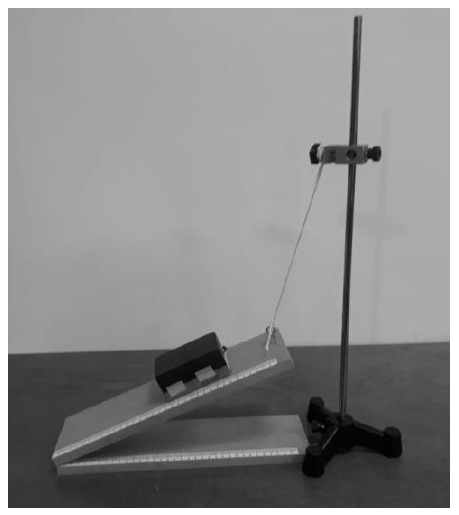
\includegraphics[width=0.95\linewidth]{static/simulados/coluni/figuras/2019/questao-24/figura-1.png}
\end{figure}
% COLUNI-AUTO-FIGURES-END

Questionados sobre as forças atuantes no bloco de madeira e, por que ele não desce, os estudantes fizeram as seguintes afirmativas:

André: A força peso está no sentido contrário à força de atrito e, por isso, o bloco não desce.

Marcela: O bloco está em repouso porque a força de atrito é maior e contrária à componente da força peso que faria o bloco escorregar.

Martha: Se não existisse atrito entre o bloco e a tábua que o suporta, o bloco escorregaria mesmo se a tábua tivesse a metade da inclinação.

\par

Estão INCORRETAS as afirmativas de:


\begin{enumerate}
\item André e Martha, apenas.
\item André e Marcela, apenas.
\item Marcela e Martha, apenas.
\item André, Marcela e Martha.\end{enumerate}
